% Options for packages loaded elsewhere
\PassOptionsToPackage{unicode}{hyperref}
\PassOptionsToPackage{hyphens}{url}
%
\documentclass[
]{article}
\usepackage{amsmath,amssymb}
\usepackage{lmodern}
\usepackage{ifxetex,ifluatex}
\ifnum 0\ifxetex 1\fi\ifluatex 1\fi=0 % if pdftex
  \usepackage[T1]{fontenc}
  \usepackage[utf8]{inputenc}
  \usepackage{textcomp} % provide euro and other symbols
\else % if luatex or xetex
  \usepackage{unicode-math}
  \defaultfontfeatures{Scale=MatchLowercase}
  \defaultfontfeatures[\rmfamily]{Ligatures=TeX,Scale=1}
\fi
% Use upquote if available, for straight quotes in verbatim environments
\IfFileExists{upquote.sty}{\usepackage{upquote}}{}
\IfFileExists{microtype.sty}{% use microtype if available
  \usepackage[]{microtype}
  \UseMicrotypeSet[protrusion]{basicmath} % disable protrusion for tt fonts
}{}
\makeatletter
\@ifundefined{KOMAClassName}{% if non-KOMA class
  \IfFileExists{parskip.sty}{%
    \usepackage{parskip}
  }{% else
    \setlength{\parindent}{0pt}
    \setlength{\parskip}{6pt plus 2pt minus 1pt}}
}{% if KOMA class
  \KOMAoptions{parskip=half}}
\makeatother
\usepackage{xcolor}
\IfFileExists{xurl.sty}{\usepackage{xurl}}{} % add URL line breaks if available
\IfFileExists{bookmark.sty}{\usepackage{bookmark}}{\usepackage{hyperref}}
\hypersetup{
  pdftitle={Curriculum Vitae},
  hidelinks,
  pdfcreator={LaTeX via pandoc}}
\urlstyle{same} % disable monospaced font for URLs
\usepackage[margin=1in]{geometry}
\usepackage{graphicx}
\makeatletter
\def\maxwidth{\ifdim\Gin@nat@width>\linewidth\linewidth\else\Gin@nat@width\fi}
\def\maxheight{\ifdim\Gin@nat@height>\textheight\textheight\else\Gin@nat@height\fi}
\makeatother
% Scale images if necessary, so that they will not overflow the page
% margins by default, and it is still possible to overwrite the defaults
% using explicit options in \includegraphics[width, height, ...]{}
\setkeys{Gin}{width=\maxwidth,height=\maxheight,keepaspectratio}
% Set default figure placement to htbp
\makeatletter
\def\fps@figure{htbp}
\makeatother
\setlength{\emergencystretch}{3em} % prevent overfull lines
\providecommand{\tightlist}{%
  \setlength{\itemsep}{0pt}\setlength{\parskip}{0pt}}
\setcounter{secnumdepth}{-\maxdimen} % remove section numbering
<!--radix_placeholder_navigation_in_header-->
<meta name="distill:offset" content=""/>

<script type="application/javascript">

  window.headroom_prevent_pin = false;

  window.document.addEventListener("DOMContentLoaded", function (event) {

    // initialize headroom for banner
    var header = $('header').get(0);
    var headerHeight = header.offsetHeight;
    var headroom = new Headroom(header, {
      tolerance: 5,
      onPin : function() {
        if (window.headroom_prevent_pin) {
          window.headroom_prevent_pin = false;
          headroom.unpin();
        }
      }
    });
    headroom.init();
    if(window.location.hash)
      headroom.unpin();
    $(header).addClass('headroom--transition');

    // offset scroll location for banner on hash change
    // (see: https://github.com/WickyNilliams/headroom.js/issues/38)
    window.addEventListener("hashchange", function(event) {
      window.scrollTo(0, window.pageYOffset - (headerHeight + 25));
    });

    // responsive menu
    $('.distill-site-header').each(function(i, val) {
      var topnav = $(this);
      var toggle = topnav.find('.nav-toggle');
      toggle.on('click', function() {
        topnav.toggleClass('responsive');
      });
    });

    // nav dropdowns
    $('.nav-dropbtn').click(function(e) {
      $(this).next('.nav-dropdown-content').toggleClass('nav-dropdown-active');
      $(this).parent().siblings('.nav-dropdown')
         .children('.nav-dropdown-content').removeClass('nav-dropdown-active');
    });
    $("body").click(function(e){
      $('.nav-dropdown-content').removeClass('nav-dropdown-active');
    });
    $(".nav-dropdown").click(function(e){
      e.stopPropagation();
    });
  });
</script>

<style type="text/css">

/* Theme (user-documented overrideables for nav appearance) */

.distill-site-nav {
  color: rgba(255, 255, 255, 0.8);
  background-color: #0F2E3D;
  font-size: 15px;
  font-weight: 300;
}

.distill-site-nav a {
  color: inherit;
  text-decoration: none;
}

.distill-site-nav a:hover {
  color: white;
}

@media print {
  .distill-site-nav {
    display: none;
  }
}

.distill-site-header {

}

.distill-site-footer {

}


/* Site Header */

.distill-site-header {
  width: 100%;
  box-sizing: border-box;
  z-index: 3;
}

.distill-site-header .nav-left {
  display: inline-block;
  margin-left: 8px;
}

@media screen and (max-width: 768px) {
  .distill-site-header .nav-left {
    margin-left: 0;
  }
}


.distill-site-header .nav-right {
  float: right;
  margin-right: 8px;
}

.distill-site-header a,
.distill-site-header .title {
  display: inline-block;
  text-align: center;
  padding: 14px 10px 14px 10px;
}

.distill-site-header .title {
  font-size: 18px;
  min-width: 150px;
}

.distill-site-header .logo {
  padding: 0;
}

.distill-site-header .logo img {
  display: none;
  max-height: 20px;
  width: auto;
  margin-bottom: -4px;
}

.distill-site-header .nav-image img {
  max-height: 18px;
  width: auto;
  display: inline-block;
  margin-bottom: -3px;
}



@media screen and (min-width: 1000px) {
  .distill-site-header .logo img {
    display: inline-block;
  }
  .distill-site-header .nav-left {
    margin-left: 20px;
  }
  .distill-site-header .nav-right {
    margin-right: 20px;
  }
  .distill-site-header .title {
    padding-left: 12px;
  }
}


.distill-site-header .nav-toggle {
  display: none;
}

.nav-dropdown {
  display: inline-block;
  position: relative;
}

.nav-dropdown .nav-dropbtn {
  border: none;
  outline: none;
  color: rgba(255, 255, 255, 0.8);
  padding: 16px 10px;
  background-color: transparent;
  font-family: inherit;
  font-size: inherit;
  font-weight: inherit;
  margin: 0;
  margin-top: 1px;
  z-index: 2;
}

.nav-dropdown-content {
  display: none;
  position: absolute;
  background-color: white;
  min-width: 200px;
  border: 1px solid rgba(0,0,0,0.15);
  border-radius: 4px;
  box-shadow: 0px 8px 16px 0px rgba(0,0,0,0.1);
  z-index: 1;
  margin-top: 2px;
  white-space: nowrap;
  padding-top: 4px;
  padding-bottom: 4px;
}

.nav-dropdown-content hr {
  margin-top: 4px;
  margin-bottom: 4px;
  border: none;
  border-bottom: 1px solid rgba(0, 0, 0, 0.1);
}

.nav-dropdown-active {
  display: block;
}

.nav-dropdown-content a, .nav-dropdown-content .nav-dropdown-header {
  color: black;
  padding: 6px 24px;
  text-decoration: none;
  display: block;
  text-align: left;
}

.nav-dropdown-content .nav-dropdown-header {
  display: block;
  padding: 5px 24px;
  padding-bottom: 0;
  text-transform: uppercase;
  font-size: 14px;
  color: #999999;
  white-space: nowrap;
}

.nav-dropdown:hover .nav-dropbtn {
  color: white;
}

.nav-dropdown-content a:hover {
  background-color: #ddd;
  color: black;
}

.nav-right .nav-dropdown-content {
  margin-left: -45%;
  right: 0;
}

@media screen and (max-width: 768px) {
  .distill-site-header a, .distill-site-header .nav-dropdown  {display: none;}
  .distill-site-header a.nav-toggle {
    float: right;
    display: block;
  }
  .distill-site-header .title {
    margin-left: 0;
  }
  .distill-site-header .nav-right {
    margin-right: 0;
  }
  .distill-site-header {
    overflow: hidden;
  }
  .nav-right .nav-dropdown-content {
    margin-left: 0;
  }
}


@media screen and (max-width: 768px) {
  .distill-site-header.responsive {position: relative; min-height: 500px; }
  .distill-site-header.responsive a.nav-toggle {
    position: absolute;
    right: 0;
    top: 0;
  }
  .distill-site-header.responsive a,
  .distill-site-header.responsive .nav-dropdown {
    display: block;
    text-align: left;
  }
  .distill-site-header.responsive .nav-left,
  .distill-site-header.responsive .nav-right {
    width: 100%;
  }
  .distill-site-header.responsive .nav-dropdown {float: none;}
  .distill-site-header.responsive .nav-dropdown-content {position: relative;}
  .distill-site-header.responsive .nav-dropdown .nav-dropbtn {
    display: block;
    width: 100%;
    text-align: left;
  }
}

/* Site Footer */

.distill-site-footer {
  width: 100%;
  overflow: hidden;
  box-sizing: border-box;
  z-index: 3;
  margin-top: 30px;
  padding-top: 30px;
  padding-bottom: 30px;
  text-align: center;
}

/* Headroom */

d-title {
  padding-top: 6rem;
}

@media print {
  d-title {
    padding-top: 4rem;
  }
}

.headroom {
  z-index: 1000;
  position: fixed;
  top: 0;
  left: 0;
  right: 0;
}

.headroom--transition {
  transition: all .4s ease-in-out;
}

.headroom--unpinned {
  top: -100px;
}

.headroom--pinned {
  top: 0;
}

/* adjust viewport for navbar height */
/* helps vertically center bootstrap (non-distill) content */
.min-vh-100 {
  min-height: calc(100vh - 100px) !important;
}

</style>

<script src="site_libs/jquery-1.11.3/jquery.min.js"></script>
<link href="site_libs/font-awesome-5.1.0/css/all.css" rel="stylesheet"/>
<link href="site_libs/font-awesome-5.1.0/css/v4-shims.css" rel="stylesheet"/>
<script src="site_libs/headroom-0.9.4/headroom.min.js"></script>
<script src="site_libs/autocomplete-0.37.1/autocomplete.min.js"></script>
<script src="site_libs/fuse-6.4.1/fuse.min.js"></script>

<script type="application/javascript">

function getMeta(metaName) {
  var metas = document.getElementsByTagName('meta');
  for (let i = 0; i < metas.length; i++) {
    if (metas[i].getAttribute('name') === metaName) {
      return metas[i].getAttribute('content');
    }
  }
  return '';
}

function offsetURL(url) {
  var offset = getMeta('distill:offset');
  return offset ? offset + '/' + url : url;
}

function createFuseIndex() {

  // create fuse index
  var options = {
    keys: [
      { name: 'title', weight: 20 },
      { name: 'categories', weight: 15 },
      { name: 'description', weight: 10 },
      { name: 'contents', weight: 5 },
    ],
    ignoreLocation: true,
    threshold: 0
  };
  var fuse = new window.Fuse([], options);

  // fetch the main search.json
  return fetch(offsetURL('search.json'))
    .then(function(response) {
      if (response.status == 200) {
        return response.json().then(function(json) {
          // index main articles
          json.articles.forEach(function(article) {
            fuse.add(article);
          });
          // download collections and index their articles
          return Promise.all(json.collections.map(function(collection) {
            return fetch(offsetURL(collection)).then(function(response) {
              if (response.status === 200) {
                return response.json().then(function(articles) {
                  articles.forEach(function(article) {
                    fuse.add(article);
                  });
                })
              } else {
                return Promise.reject(
                  new Error('Unexpected status from search index request: ' +
                            response.status)
                );
              }
            });
          })).then(function() {
            return fuse;
          });
        });

      } else {
        return Promise.reject(
          new Error('Unexpected status from search index request: ' +
                      response.status)
        );
      }
    });
}

window.document.addEventListener("DOMContentLoaded", function (event) {

  // get search element (bail if we don't have one)
  var searchEl = window.document.getElementById('distill-search');
  if (!searchEl)
    return;

  createFuseIndex()
    .then(function(fuse) {

      // make search box visible
      searchEl.classList.remove('hidden');

      // initialize autocomplete
      var options = {
        autoselect: true,
        hint: false,
        minLength: 2,
      };
      window.autocomplete(searchEl, options, [{
        source: function(query, callback) {
          const searchOptions = {
            isCaseSensitive: false,
            shouldSort: true,
            minMatchCharLength: 2,
            limit: 10,
          };
          var results = fuse.search(query, searchOptions);
          callback(results
            .map(function(result) { return result.item; })
          );
        },
        templates: {
          suggestion: function(suggestion) {
            var img = suggestion.preview && Object.keys(suggestion.preview).length > 0
              ? `<img src="${offsetURL(suggestion.preview)}"</img>`
              : '';
            var html = `
              <div class="search-item">
                <h3>${suggestion.title}</h3>
                <div class="search-item-description">
                  ${suggestion.description || ''}
                </div>
                <div class="search-item-preview">
                  ${img}
                </div>
              </div>
            `;
            return html;
          }
        }
      }]).on('autocomplete:selected', function(event, suggestion) {
        window.location.href = offsetURL(suggestion.path);
      });
      // remove inline display style on autocompleter (we want to
      // manage responsive display via css)
      $('.algolia-autocomplete').css("display", "");
    })
    .catch(function(error) {
      console.log(error);
    });

});

</script>

<style type="text/css">

.nav-search {
  font-size: x-small;
}

/* Algolioa Autocomplete */

.algolia-autocomplete {
  display: inline-block;
  margin-left: 10px;
  vertical-align: sub;
  background-color: white;
  color: black;
  padding: 6px;
  padding-top: 8px;
  padding-bottom: 0;
  border-radius: 6px;
  border: 1px #0F2E3D solid;
  width: 180px;
}


@media screen and (max-width: 768px) {
  .distill-site-nav .algolia-autocomplete {
    display: none;
    visibility: hidden;
  }
  .distill-site-nav.responsive .algolia-autocomplete {
    display: inline-block;
    visibility: visible;
  }
  .distill-site-nav.responsive .algolia-autocomplete .aa-dropdown-menu {
    margin-left: 0;
    width: 400px;
    max-height: 400px;
  }
}

.algolia-autocomplete .aa-input, .algolia-autocomplete .aa-hint {
  width: 90%;
  outline: none;
  border: none;
}

.algolia-autocomplete .aa-hint {
  color: #999;
}
.algolia-autocomplete .aa-dropdown-menu {
  width: 550px;
  max-height: 70vh;
  overflow-x: visible;
  overflow-y: scroll;
  padding: 5px;
  margin-top: 3px;
  margin-left: -150px;
  background-color: #fff;
  border-radius: 5px;
  border: 1px solid #999;
  border-top: none;
}

.algolia-autocomplete .aa-dropdown-menu .aa-suggestion {
  cursor: pointer;
  padding: 5px 4px;
  border-bottom: 1px solid #eee;
}

.algolia-autocomplete .aa-dropdown-menu .aa-suggestion:last-of-type {
  border-bottom: none;
  margin-bottom: 2px;
}

.algolia-autocomplete .aa-dropdown-menu .aa-suggestion .search-item {
  overflow: hidden;
  font-size: 0.8em;
  line-height: 1.4em;
}

.algolia-autocomplete .aa-dropdown-menu .aa-suggestion .search-item h3 {
  font-size: 1rem;
  margin-block-start: 0;
  margin-block-end: 5px;
}

.algolia-autocomplete .aa-dropdown-menu .aa-suggestion .search-item-description {
  display: inline-block;
  overflow: hidden;
  height: 2.8em;
  width: 80%;
  margin-right: 4%;
}

.algolia-autocomplete .aa-dropdown-menu .aa-suggestion .search-item-preview {
  display: inline-block;
  width: 15%;
}

.algolia-autocomplete .aa-dropdown-menu .aa-suggestion .search-item-preview img {
  height: 3em;
  width: auto;
  display: none;
}

.algolia-autocomplete .aa-dropdown-menu .aa-suggestion .search-item-preview img[src] {
  display: initial;
}

.algolia-autocomplete .aa-dropdown-menu .aa-suggestion.aa-cursor {
  background-color: #eee;
}
.algolia-autocomplete .aa-dropdown-menu .aa-suggestion em {
  font-weight: bold;
  font-style: normal;
}

</style>


<!--/radix_placeholder_navigation_in_header-->
<!--radix_placeholder_site_in_header-->
<!--/radix_placeholder_site_in_header-->

<style type="text/css">
body {
  padding-top: 60px;
}
</style>
<style type="text/css">
/* base variables */

/* Edit the CSS properties in this file to create a custom
   Distill theme. Only edit values in the right column
   for each row; values shown are the CSS defaults.
   To return any property to the default,
   you may set its value to: unset
   All rows must end with a semi-colon.                      */

/* Optional: embed custom fonts here with `@import`          */
/* This must remain at the top of this file.                 */



html {
  /*-- Main font sizes --*/
  --title-size:      50px;
  --body-size:       1.06rem;
  --code-size:       14px;
  --aside-size:      12px;
  --fig-cap-size:    13px;
  /*-- Main font colors --*/
  --title-color:     #000000;
  --header-color:    rgba(0, 0, 0, 0.8);
  --body-color:      rgba(0, 0, 0, 0.8);
  --aside-color:     rgba(0, 0, 0, 0.6);
  --fig-cap-color:   rgba(0, 0, 0, 0.6);
  /*-- Specify custom fonts ~~~ must be imported above   --*/
  --heading-font:    sans-serif;
  --mono-font:       monospace;
  --body-font:       sans-serif;
  --navbar-font:     sans-serif;  /* websites + blogs only */
}

/*-- ARTICLE METADATA --*/
d-byline {
  --heading-size:    0.6rem;
  --heading-color:   rgba(0, 0, 0, 0.5);
  --body-size:       0.8rem;
  --body-color:      rgba(0, 0, 0, 0.8);
}

/*-- ARTICLE TABLE OF CONTENTS --*/
.d-contents {
  --heading-size:    18px;
  --contents-size:   13px;
}

/*-- ARTICLE APPENDIX --*/
d-appendix {
  --heading-size:    15px;
  --heading-color:   rgba(0, 0, 0, 0.65);
  --text-size:       0.8em;
  --text-color:      rgba(0, 0, 0, 0.5);
}

/*-- WEBSITE HEADER + FOOTER --*/
/* These properties only apply to Distill sites and blogs  */

.distill-site-header {
  --title-size:       18px;
  --text-color:       rgba(255, 255, 255, 0.8);
  --text-size:        15px;
  --hover-color:      white;
  --bkgd-color:       #0F2E3D;
}

.distill-site-footer {
  --text-color:       rgba(255, 255, 255, 0.8);
  --text-size:        15px;
  --hover-color:      white;
  --bkgd-color:       #0F2E3D;
}

/*-- Additional custom styles --*/
/* Add any additional CSS rules below                      */
</style>
<style type="text/css">/* base variables */

/* Edit the CSS properties in this file to create a custom
   Distill theme. Only edit values in the right column
   for each row; values shown are the CSS defaults.
   To return any property to the default,
   you may set its value to: unset
   All rows must end with a semi-colon.                      */

/* Optional: embed custom fonts here with `@import`          */
/* This must remain at the top of this file.                 */
@import url('https://fonts.googleapis.com/css2?family=Open+Sans');


html {
  /*-- Main font sizes --*/
  --title-size:      30px;
  --body-size:       1.06rem;
  --code-size:       14px;
  --aside-size:      12px;
  --fig-cap-size:    13px;
  /*-- Main font colors --*/
  --title-color:     #000000;
  --header-color:    rgba(0, 0, 0, 0.8);
  --body-color:      rgba(0, 0, 0, 0.8);
  --aside-color:     rgba(0, 0, 0, 0.6);
  --fig-cap-color:   rgba(0, 0, 0, 0.6);
  /*-- Specify custom fonts ~~~ must be imported above   --*/
  --heading-font:    open-sans;
  --mono-font:       monospace;
  --body-font:       open-sans;
  --navbar-font:     open-sans;  /* websites + blogs only */
}

/*-- ARTICLE METADATA --*/
d-byline {
  --heading-size:    0.6rem;
  --heading-color:   #636363;
  --body-size:       0.8rem;
  --body-color:      #636363;
}

/*-- ARTICLE TABLE OF CONTENTS --*/
.d-contents {
  --heading-size:    18px;
  --contents-size:   13px;
}

/*-- ARTICLE APPENDIX --*/
d-appendix {
  --heading-size:    15px;
  --heading-color:   #636363;
  --text-size:       0.8em;
  --text-color:      #636363;
}

/*-- WEBSITE HEADER + FOOTER --*/
/* These properties only apply to Distill sites and blogs  */

.distill-site-header {
  --title-size:       18px;
  --text-color:       #636363;
  --text-size:        15px;
  --hover-color:      black;
  --bkgd-color:       white;
}

.distill-site-footer {
  --text-color:       #636363;
  --text-size:        15px;
  --hover-color:      black;
  --bkgd-color:       white;
}

/*-- Additional custom styles --*/
/* Add any additional CSS rules below                      */
</style>
<style type="text/css">
/* base style */

/* FONT FAMILIES */

:root {
  --heading-default: -apple-system, BlinkMacSystemFont, "Segoe UI", Roboto, Oxygen, Ubuntu, Cantarell, "Fira Sans", "Droid Sans", "Helvetica Neue", Arial, sans-serif;
  --mono-default: Consolas, Monaco, 'Andale Mono', 'Ubuntu Mono', monospace;
  --body-default: -apple-system, BlinkMacSystemFont, "Segoe UI", Roboto, Oxygen, Ubuntu, Cantarell, "Fira Sans", "Droid Sans", "Helvetica Neue", Arial, sans-serif;
}

body,
.posts-list .post-preview p,
.posts-list .description p {
  font-family: var(--body-font), var(--body-default);
}

h1, h2, h3, h4, h5, h6,
.posts-list .post-preview h2,
.posts-list .description h2 {
  font-family: var(--heading-font), var(--heading-default);
}

d-article div.sourceCode code,
d-article pre code {
  font-family: var(--mono-font), var(--mono-default);
}


/*-- TITLE --*/
d-title h1,
.posts-list > h1 {
  color: var(--title-color, black);
}

d-title h1 {
  font-size: var(--title-size, 50px);
}

/*-- HEADERS --*/
d-article h1,
d-article h2,
d-article h3,
d-article h4,
d-article h5,
d-article h6 {
  color: var(--header-color, rgba(0, 0, 0, 0.8));
}

/*-- BODY --*/
d-article > p,  /* only text inside of <p> tags */
d-article > ul, /* lists */
d-article > ol {
  color: var(--body-color, rgba(0, 0, 0, 0.8));
  font-size: var(--body-size, 1.06rem);
}


/*-- CODE --*/
d-article div.sourceCode code,
d-article pre code {
  font-size: var(--code-size, 14px);
}

/*-- ASIDE --*/
d-article aside {
  font-size: var(--aside-size, 12px);
  color: var(--aside-color, rgba(0, 0, 0, 0.6));
}

/*-- FIGURE CAPTIONS --*/
figure .caption,
figure figcaption,
.figure .caption {
  font-size: var(--fig-cap-size, 13px);
  color: var(--fig-cap-color, rgba(0, 0, 0, 0.6));
}

/*-- METADATA --*/
d-byline h3 {
  font-size: var(--heading-size, 0.6rem);
  color: var(--heading-color, rgba(0, 0, 0, 0.5));
}

d-byline {
  font-size: var(--body-size, 0.8rem);
  color: var(--body-color, rgba(0, 0, 0, 0.8));
}

d-byline a,
d-article d-byline a {
  color: var(--body-color, rgba(0, 0, 0, 0.8));
}

/*-- TABLE OF CONTENTS --*/
.d-contents nav h3 {
  font-size: var(--heading-size, 18px);
}

.d-contents nav a {
  font-size: var(--contents-size, 13px);
}

/*-- APPENDIX --*/
d-appendix h3 {
  font-size: var(--heading-size, 15px);
  color: var(--heading-color, rgba(0, 0, 0, 0.65));
}

d-appendix {
  font-size: var(--text-size, 0.8em);
  color: var(--text-color, rgba(0, 0, 0, 0.5));
}

d-appendix d-footnote-list a.footnote-backlink {
  color: var(--text-color, rgba(0, 0, 0, 0.5));
}

/*-- WEBSITE HEADER + FOOTER --*/
.distill-site-header .title {
  font-size: var(--title-size, 18px);
  font-family: var(--navbar-font), var(--heading-default);
}

.distill-site-header a,
.nav-dropdown .nav-dropbtn {
  font-family: var(--navbar-font), var(--heading-default);
}

.nav-dropdown .nav-dropbtn {
  color: var(--text-color, rgba(255, 255, 255, 0.8));
  font-size: var(--text-size, 15px);
}

.distill-site-header a:hover,
.nav-dropdown:hover .nav-dropbtn {
  color: var(--hover-color, white);
}

.distill-site-header {
  font-size: var(--text-size, 15px);
  color: var(--text-color, rgba(255, 255, 255, 0.8));
  background-color: var(--bkgd-color, #0F2E3D);
}

.distill-site-footer {
  font-size: var(--text-size, 15px);
  color: var(--text-color, rgba(255, 255, 255, 0.8));
  background-color: var(--bkgd-color, #0F2E3D);
}

.distill-site-footer a:hover {
  color: var(--hover-color, white);
}</style>
\ifluatex
  \usepackage{selnolig}  % disable illegal ligatures
\fi

\title{Curriculum Vitae}
\author{}
\date{\vspace{-2.5em}}

\begin{document}
\maketitle

<!--radix_placeholder_navigation_before_body-->
<header class="header header--fixed" role="banner">
<nav class="distill-site-nav distill-site-header">
<div class="nav-left">
<a href="index.html" class="title">Jae-Young Son</a>
<a href="cv.html">CV</a>
<a href="publications.html">Publications</a>
<a href="blog.html">PsychBlog &amp; Jelly</a>
<div class="nav-dropdown">
<button class="nav-dropbtn">
External
 
<span class="down-arrow">&#x25BE;</span>
</button>
<div class="nav-dropdown-content">
<a href="https://twitter.com/psychNerdJae">Twitter</a>
<a href="https://github.com/psychNerdJae">GitHub</a>
<a href="https://scholar.google.com/citations?user=JPPuzI8AAAAJ">Google Scholar</a>
<a href="https://neurotree.org/neurotree/tree.php?pid=747308">NeuroTree</a>
</div>
</div>
<input id="distill-search" class="nav-search hidden" type="text" placeholder="Search..."/>
</div>
<div class="nav-right">
<a href="javascript:void(0);" class="nav-toggle">&#9776;</a>
</div>
</nav>
</header>
<!--/radix_placeholder_navigation_before_body-->

<!--radix_placeholder_site_before_body-->
<!--/radix_placeholder_site_before_body-->

\hypertarget{jae-young-son}{%
\section{Jae-Young Son}\label{jae-young-son}}

\href{https://jaeyoungson.com/cv.pdf}{\textbf{Download CV}} \textbar{}
\href{https://scholar.google.com/citations?user=JPPuzI8AAAAJ}{\textbf{Google
Scholar}}

\textbf{Email:} jae at brown dot edu \textbar{} \textbf{Website:}
\href{https://jaeyoungson.com}{www.jaeyoungson.com}

This document was most recently compiled on 2021-03-24 using R Markdown.

\hypertarget{education}{%
\section{Education}\label{education}}

\textbf{Ph.D.}\\
Brown University\\
Dept. of Cognitive, Linguistic, \& Psychological Sciences (CLPS)\\
2018 - Present\\
Advisor: Oriel FeldmanHall

\textbf{B.A.}\\
Stanford University\\
2012 - 2016\\
Psychology major advisor: Jamil Zaki\\
Neuroscience concentration advisor: Samuel McClure

\hypertarget{employment}{%
\section{Employment}\label{employment}}

\textbf{Lab Manager}\\
2016 - 2018\\
Brown University\\
Dept. of Cognitive, Linguistic, \& Psychological Sciences (CLPS)\\
Supervisor: Oriel FeldmanHall\\

\textbf{Research Assistant}\\
2013 - 2016\\
Stanford University\\
Dept. of Psychology\\
Supervisors: Jamil Zaki \& W. Craig Williams

\hypertarget{publications}{%
\section{Publications}\label{publications}}

\begin{enumerate}
\def\labelenumi{\arabic{enumi}.}
\item
  \textbf{Son, J.}, Bhandari, A., \& FeldmanHall, O. (revise \&
  resubmit). Cognitive maps of social features enable adaptive inference
  in social networks.
\item
  Heffner, J., \textbf{Son, J.}, \& FeldmanHall, O. (revise \&
  resubmit). Emotion prediction errors guide socially adaptive behavior.
\item
  \textbf{Son, J.}, Bhandari, A., \& FeldmanHall, O. (2019).
  Crowdsourcing punishment: Individuals reference group preferences to
  inform their own punitive decisions. \emph{Scientific Reports.}
  \href{https://www.nature.com/articles/s41598-019-48050-2}{\textbf{Online}}
  \textbar{}
  \href{https://github.com/psychNerdJae/psychnerdjae.github.io/blob/main/papers/CrowdsourcingPunishment_SciRep_2019.pdf?raw=true}{\textbf{PDF}}
  \textbar{} \href{https://osf.io/8ka47/}{\textbf{Data}}
\item
  FeldmanHall, O., \textbf{Son, J.}, \& Heffner, J. (2018). Norms and
  the flexibility of moral action. \emph{Personality Neuroscience.}
  \href{https://www.cambridge.org/core/journals/personality-neuroscience/article/norms-and-the-flexibility-of-moral-action/A8A5140A517ECEE314A21FF9FE0E9EED}{\textbf{Online}}
  \textbar{}
  \href{https://github.com/psychNerdJae/psychnerdjae.github.io/blob/main/papers/NormsMoralAction_PN_2018.pdf?raw=true}{\textbf{PDF}}
\end{enumerate}

\emph{Disclaimer: The PDFs provided may be copyrighted by the
journals/edited volumes in which they are published. Access to these
articles is provided to facilitate timely distribution of scientific
knowledge, and is therefore intended for your personal use only. No
commercial use may be made of these articles, nor is mass production of
these articles permitted.}

\hypertarget{talks}{%
\section{Talks}\label{talks}}

\begin{enumerate}
\def\labelenumi{\arabic{enumi}.}
\item
  \textbf{Son, J.} (December 2019). Crowdsourcing punishment:
  Individuals reference group preferences to inform their own punitive
  decisions. Presented at the Brown University Social Cognitive Seminar
  Series, Providence, RI.
\item
  \textbf{Son, J.} (October 2019). How do people use structure to learn
  about social networks? Presented at the Brown University First Year
  Presentation Colloquium, Providence, RI.
\item
  \textbf{Son, J.} (June 2019). Structure learning in social networks.
  Presented at the 3rd Annual Meeting of New England Research on
  Decision-Making, Cambridge MA.
\item
  \textbf{Son, J.} (March 2018). How groups exert influence over
  decision-making. Talk given at a lab meeting for the Morality Lab at
  Boston College, Boston, MA.
\item
  \textbf{Son, J.}, \& FeldmanHall, O. (May 2017). A tipping-point
  conformity effect for justice: Group choice shifts preferences for
  punishment. Talk given at the 1st Annual Meeting of NERD (New England
  Research on Decision-Making), Providence, RI.
\item
  \textbf{Son, J.}, Tamir, D.I., Williams, W.C., \& Zaki, J. (June
  2016). Preferences for gathering and sharing social information about
  the self and friends: Disclosure target and directionality predict
  disclosure choice. Talk given at the Annual Stanford Psychology Honors
  Colloquium, Stanford, CA.
\end{enumerate}

\hypertarget{posters}{%
\section{Posters}\label{posters}}

\emph{* Indicates mentored student}

\begin{enumerate}
\def\labelenumi{\arabic{enumi}.}
\item
  \textbf{Son, J.}, Bhandari, A., \& FeldmanHall, O. (October 2020).
  Structural knowledge adaptively shapes the representation of social
  networks. Presented at the 18th Annual Meeting of the Society for
  NeuroEconomics (virtual).
\item
  \textbf{Son, J.}, Bhandari, A., \& FeldmanHall, O. (March 2019).
  Crowdsourcing punishment: Individuals reference group preferences to
  inform their own punitive decisions. Poster presented at the 6th
  Annual Meeting of the Society for Affective Science, Boston, MA.
\item
  Heffner, J., \textbf{Son, J.}, \& FeldmanHall, O. (March 2018).
  Emotion prediction errors predict decisions to punish. Poster
  presented at the 21st Annual Mind/Brain Research Day, Providence, RI.
\item
  Lee, W.*, \textbf{Son, J.}, \& FeldmanHall, O. (March 2018). Social
  influence increases preferences for uncertain gambles. Poster
  presented at the 21st Annual Mind/Brain Research Day, Providence, RI.
\item
  Hu, M.*, \textbf{Son, J.}, \& FeldmanHall, O. (August 2017). Acquired
  equivalence: Evidence for mechanisms supporting moral learning. Poster
  presented at the annual Brown Summer Research Symposium, Providence,
  RI.
\item
  \textbf{Son, J.}, \& FeldmanHall, O. (May 2017). A tipping-point
  conformity effect for justice: Group choice shifts preferences for
  punishment. Poster presented at the 29th Annual Meeting of the
  Association for Psychological Science, Boston, MA.
\item
  \textbf{Son, J.}, \& FeldmanHall, O. (March 2017). A tipping-point
  conformity effect for justice: Group choice shifts preferences for
  punishment. Poster presented at the 20th Annual Mind/Brain Research
  Day, Providence, RI.
\item
  Williams, W.C., Leong, Y.C., \textbf{Son, J.}, Alqueza, K., \& Zaki,
  J. (April 2016). Facial expressions track brain regions associated
  with affective salience and theory of mind. Poster presented at the
  9th Annual Meeting of the Social \& Affective Neuroscience Society,
  New York, NY.
\item
  Williams, W.C., Leong, Y.C., \textbf{Son, J.}, Alqueza, K., \& Zaki,
  J. (March 2016). Facial expressions track brain regions associated
  with affective salience and theory of mind. Poster presented at the
  3rd Annual Meeting of the Society for Affective Science, Chicago, IL.
\item
  Williams, W.C., Leong, Y.C., \textbf{Son, J.}, Alqueza, K., \& Zaki,
  J. (January 2016). Facial expressions track brain regions associated
  with affective salience and theory of mind. Poster presented at the
  17th Annual Emotion Pre-Conference to the Annual Meeting of the
  Society for Personality and Social Psychology, San Diego, CA.
\item
  Williams, W.C., Nook, E., \textbf{Son, J.}, \& Zaki, J. (April 2014).
  Audiences enhance the expression and communication but not the
  experience of emotion. Poster presented at the 7th Annual Meeting of
  the Social \& Affective Neuroscience Society, Denver, CO.
\item
  Williams, W.C., Nook, E., \textbf{Son, J.}, \& Zaki, J. (February
  2014). Audiences enhance the expression and communication but not the
  experience of emotion. Poster presented at the 9th Annual Emotion
  Pre-Conference to the Annual Meeting of the Society for Personality
  and Social Psychology, Austin, TX.
\item
  Williams, W.C., Nook, E., \textbf{Son, J.}, \& Zaki, J. (June 2013).
  Audiences enhance the expression and communication but not the
  experience of emotion. Poster presented at the Stanford PsychSummer
  Conference.
\end{enumerate}

\hypertarget{grants-fellowships}{%
\section{Grants \& Fellowships}\label{grants-fellowships}}

\begin{itemize}
\item
  2019-2022 - National Science Foundation Graduate Research Fellowship
  Program (\$138,000, award \#2040433)
\item
  2019 - Brown University Graduate Travel Grant (\$622)
\item
  2015 - Stanford Undergraduate Advising \& Research ``Small Grant''
  (\$1,500)
\item
  2014 - Stanford Undergraduate Teaching Fellowship (\$1,000)
\item
  2013 - Stanford PsychSummer Grant (\$7,500)
\end{itemize}

\hypertarget{awards-honors}{%
\section{Awards \& Honors}\label{awards-honors}}

\begin{itemize}
\item
  2016 - B.A. Psychology with Departmental Honors
\item
  2013 - Stanford PsychSummer ``Best of Show'' Poster Award
\end{itemize}

\hypertarget{research-training}{%
\section{Research Training}\label{research-training}}

\begin{itemize}
\item
  2019 - Methods in Neuroscience at Dartmouth (MIND)

  \begin{itemize}
  \tightlist
  \item
    Dartmouth College, Hanover, NH
  \item
    ``Hackathon''-style summer school for computational modeling.
  \end{itemize}
\item
  2017 - Computational Modeling Workshop, Brown Institute for Brain
  Science

  \begin{itemize}
  \tightlist
  \item
    Brown University, Providence, RI
  \item
    ``Bootcamp''-style summer course covering computational modeling
    techniques such as reinforcement learning, drift diffusion modeling,
    and hierarchical Bayesian estimation.
  \end{itemize}
\end{itemize}

\hypertarget{teaching}{%
\section{Teaching}\label{teaching}}

\begin{itemize}
\item
  2020

  \begin{itemize}
  \item
    Teaching Assistant - CLPS 0700: Social Psychology

    \begin{itemize}
    \tightlist
    \item
      Brown University, Providence, RI
    \item
      Supervisor: Oriel FeldmanHall
    \item
      Introductory lecture course with an enrollment of 300 students.
      Helped students design and analyze their own studies, and provided
      guidance and feedback on writing journal-style scientific reports.
      Delivered solo guest lecture on attribution.
    \end{itemize}
  \item
    Guest Workshop Instructor - Computational Modeling Workshop, Carney
    Institute for Brain Science

    \begin{itemize}
    \tightlist
    \item
      Brown University, Providence, RI
    \item
      Delivered a hands-on workshop for estimating hierarchical drift
      diffusion models using the HDDM package in Python.
    \end{itemize}
  \end{itemize}
\item
  2019

  \begin{itemize}
  \item
    Teaching Assistant - CLPS 1790: Personality and Clinical Asessment

    \begin{itemize}
    \tightlist
    \item
      Brown University, Providence, RI
    \item
      Supervisor: Jack Wright
    \item
      Upper-level lab course with an enrollment of 24 students. Helped
      students design and analyze their own studies, and provided
      guidance and feedback on writing journal-style scientific reports.
    \end{itemize}
  \item
    Workshop Instructor - Data Science Using R

    \begin{itemize}
    \tightlist
    \item
      Brown University, Providence, RI
    \item
      Weekly workshop for undergraduates. Covered data wrangling,
      visualization, and mixed-effects regression.
    \end{itemize}
  \item
    Guest Workshop Instructor - Computational Modeling Workshop, Carney
    Institute for Brain Science

    \begin{itemize}
    \tightlist
    \item
      Brown University, Providence, RI
    \item
      Delivered a hands-on workshop for estimating hierarchical drift
      diffusion models using the HDDM package in Python.
    \end{itemize}
  \item
    Guest Lecturer - Summer @ Brown

    \begin{itemize}
    \tightlist
    \item
      Brown University, Providence, RI
    \item
      Delivered a lecture entitled ``Social Preferences and the Brain''
      for the class ``Neuroeconomics: The science of decision-making'',
      which was part of the ``Summer @ Brown'' summer school for high
      school students.
    \end{itemize}
  \end{itemize}
\item
  2018

  \begin{itemize}
  \item
    Workshop Instructor - Programming Psychology Experiments

    \begin{itemize}
    \tightlist
    \item
      Brown University, Providence, RI
    \item
      Three-part workshop teaching the fundamentals of programming
      computerized psychology experiments using PsychToolbox.
    \end{itemize}
  \end{itemize}
\item
  2014-2016

  \begin{itemize}
  \item
    Teaching Fellow - Psych One: Introduction to Psychology

    \begin{itemize}
    \tightlist
    \item
      Stanford University, Stanford, CA
    \item
      Supervisors: Bridgette Martin-Hard, James Gross, Jamil Zaki, \&
      Gregory Walton
    \item
      Taught weekly sections (13-15 students each)
    \end{itemize}
  \end{itemize}
\end{itemize}

\hypertarget{scientific-community-outreach}{%
\section{Scientific \& Community
Outreach}\label{scientific-community-outreach}}

\begin{itemize}
\item
  2021

  \begin{itemize}
  \item
    Study Group Mentor - Leadership Alliance

    \begin{itemize}
    \tightlist
    \item
      Provided mentorship for undergraduate students (the Carney Brain
      Science cohort) participating in Leadership Alliance, an
      organization that provides research opportunities to students from
      historically underrepresented and marginalized groups.
    \end{itemize}
  \item
    Lesson Plan Designer - Brain Week Rhode Island

    \begin{itemize}
    \tightlist
    \item
      Helped design a lesson plan to introduce Rhode Island students to
      the brain sciences, and specifically to the science of
      ingroup/outgroup cognition. Created a video introducing the
      Robber's Cave study and encouraging students to reflect on how
      groups affect their own social interactions.
    \end{itemize}
  \end{itemize}
\item
  2020

  \begin{itemize}
  \item
    Study Group Mentor - Leadership Alliance

    \begin{itemize}
    \tightlist
    \item
      Provided mentorship for undergraduate students (the Carney Brain
      Science cohort) participating in Leadership Alliance, an
      organization that provides research opportunities to students from
      historically underrepresented and marginalized groups.
    \end{itemize}
  \end{itemize}
\item
  2019

  \begin{itemize}
  \item
    Guest Workshop Instructor - Leadership Alliance

    \begin{itemize}
    \tightlist
    \item
      Delivered workshop to students participating in Leadership
      Alliance, an organization that provides research opportunities to
      students from historically underrepresented and marginalized
      groups. Discussed and practiced the principles of effective
      scientific writing and communication.
    \end{itemize}
  \end{itemize}
\item
  2016

  \begin{itemize}
  \item
    Co-organizer - Stanford Undergraduate Psychology Conference

    \begin{itemize}
    \tightlist
    \item
      An entirely undergraduate-organized conference hosted at Stanford
      University, featuring research from undergraduates from around the
      U.S. and internationally.
    \end{itemize}
  \end{itemize}
\item
  2014-2016

  \begin{itemize}
  \item
    Organizer - Stanford Undergraduate Psychology Association

    \begin{itemize}
    \item
      Generally: organized events for undergraduate students and
      community members to learn about (and engage in) psychological
      science.
    \item
      Primary organizer for a discussion with Dr.~Albert Bandura
      regarding his newly-published book, \emph{Moral Disengagement}.
    \item
      Co-organizer for a screening of the film \emph{The Stanford Prison
      Experiment}, and a panel discussion with Dr.~Philip Zimbardo
      afterwards.
    \end{itemize}
  \end{itemize}
\end{itemize}

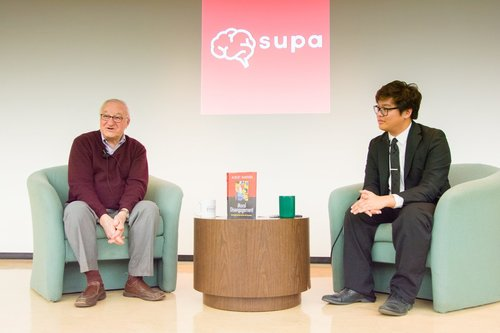
\includegraphics[height=150px]{images/bandura}
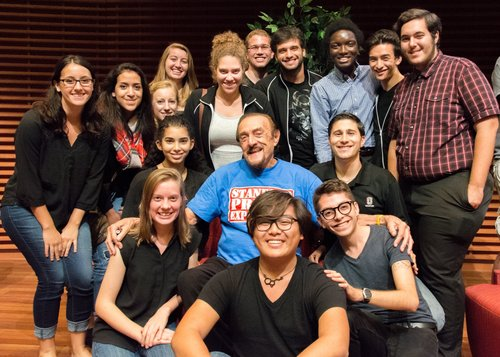
\includegraphics[height=150px]{images/zimbardo}

\hypertarget{professional-departmental-service}{%
\section{Professional \& Departmental
Service}\label{professional-departmental-service}}

\begin{itemize}
\tightlist
\item
  2020-present - Graduate Student Representative - Carney Institute for
  Brain Science
\item
  2019-present - Member of Diversity \& Innovation Committee - Society
  for Affective Science Student Committee
\item
  2019-2020 - Social Media Editor - Personality Neuroscience, Cambridge
  University Press
\item
  2019-2020 - Graduate Student Representative - Brown Dept. of Cog.,
  Ling., \& Psych. Sci.
\item
  2018-2019 - Social Events Planning Co-chair - Brown Dept. of Cog.,
  Ling., \& Psych. Sci.
\item
  2017 - Co-organizer - New England Research on Decision-Making
\end{itemize}

\hypertarget{ad-hoc-review}{%
\section{Ad Hoc Review}\label{ad-hoc-review}}

\begin{itemize}
\tightlist
\item
  Cognition
\item
  Journal of Experimental Psychology: General (JEPG)
\item
  Social, Cognitive, and Affective Neuroscience (SCAN)
\end{itemize}

\hypertarget{popular-science-writing}{%
\section{``Popular Science'' Writing}\label{popular-science-writing}}

\begin{itemize}
\item
  Carney Institute for Brain Science

  \begin{itemize}
  \tightlist
  \item
    2019:
    \href{https://www.brown.edu/carney/news/2019/02/13/what-love-here\%E2\%80\%99s-what-brain-science-can-tell-us}{What
    is love? Here's what brain science can tell us.}
  \end{itemize}
\end{itemize}

\hypertarget{media-coverage}{%
\section{Media Coverage}\label{media-coverage}}

\begin{itemize}
\item
  Brown Daily Herald

  \begin{itemize}
  \tightlist
  \item
    2018:
    \href{https://www.browndailyherald.com/2018/09/17/feldmanhall-lab-demystifies-human-behavior/}{FeldmanHall
    Lab demystifies human behavior}
  \item
    2017:
    \href{https://www.browndailyherald.com/2017/02/06/new-lab-studies-emotional-decision-making/}{New
    lab studies emotional decision-making}
  \end{itemize}
\end{itemize}

<!--radix_placeholder_site_after_body-->
<!--/radix_placeholder_site_after_body-->

<!--radix_placeholder_navigation_after_body-->
<!--/radix_placeholder_navigation_after_body-->

\end{document}
